\section{Materials and methods}
For this study, we generated molecular docking scores for two targets, AA2AR and CB2 (datasets AA2AR\_1/2 and CB2\_1/2), and also used datasets available in open-source \cite{ultralarge_docking_first} (datasets AmpC and D4). For AA2AR and CB2, we used AA2AR\_1 and CB2\_1 for most of the studies in this paper, and used docking scores from AA2AR\_2 and CB2\_2 as upper-bond baselines, implying that a docking itself (with a different random seed) is the best predictor for the docking result. Distribution of the scores from all six datasets is shown on figure \ref{fig:fig_1_distribution}.

In this work, we explored capabilities of different ML algorithms in two scenarios. First, we trained regression models on molecular fingerprints and respective docking scores, and estimated the ability of regressors to predict docking score of a molecule from its binary fingerprint. Second, we explored parameters of \textit{iterative} models: after a first train-predict round, ligands with the best predicted docking score were subjected to docking again, and a new model is trained on their docking scores. We then tested these models in their ability to recover top-1\% of the ligands, ranked by their docking score.


\subsection{Molecular docking and fingerprint generation}
To obtain the scores for AA2AR\_1/2 and CB2\_1/2, we performed molecular docking in ICM-Pro molecular modeling software (ver. 3.9.1) \cite{molsoft_guide}. We used X-ray crystal structures of CB2 (PDB ID 5ZTY, resolution 2.8 \AA) and AA2AR (PDB ID 4EIY, resolution 1.8 \AA). Models were prepared in accordance with the Molsoft ICM user guide \cite{molsoft_guide}. Namely, the files were loaded into the ICM-Pro package, ligands removed, and the receptor models converted into the ICM format using default settings, which included building of missing side chains, adding hydrogens, energy-based Gln/Asn/His conformation optimization, and removal of all water molecules. Docking box was selected within 5 \AA \ of the co-crystallized ligands in the orthosteric pocket. As a screening library, we used randomly selected $1\ 000\ 000$ drug-like (molecular weight between 200 and 500 Da, logP less than 5.0) compounds from ZINC20 database \cite{Irwin2020ZINC20Discovery}. Using ICM-Pro we converted compounds from SMILES to three-dimensional SDF  format, added hydrogen atoms and assigned formal charges at pH=7.0 (according to the pKa model implemented in ICM-Pro). Docking was performed using ICM-Pro package (ver. 3.9-1b) without receptor flexibility, and with ligand sampling thoroughness (effort) 1.0. Scoring was done with the ICM empirical scoring function \cite{abagyan_biased_1994}. Docking score values for the best ligand pose were then obtained from the resulting SDF files.


To obtain the docking scores for AmpC and D4 targets, we used the published docking scores \cite{ultralarge_docking_first} and randomly selected $1\ 000\ 000$ molecules from the full datasets provided on Figshare \cite{ultralarge_docking_first}. The scores, in turn, were earlier generated by the authors using the physics-based DOCK3.7 scoring function \cite{Coleman2013}.

In order to vectorize molecules for subsequent ML tasks, we generated Morgan fingerprints (size 2048, radius 2) using chemfp \cite{Dalke2019} for all molecules from their SMILES strings. Fingerprint radius and size were chosen as a compromise between in-memory dataset size and fingerprint performance in docking score prediction tasks \cite{logistic_regression}.

Subsequently, we use molecular fingerprints as features \texttt{X}, and docking scores for target \texttt{y}, and do not use the predicted docking poses altogether.

\begin{figure}[ht]
\centering
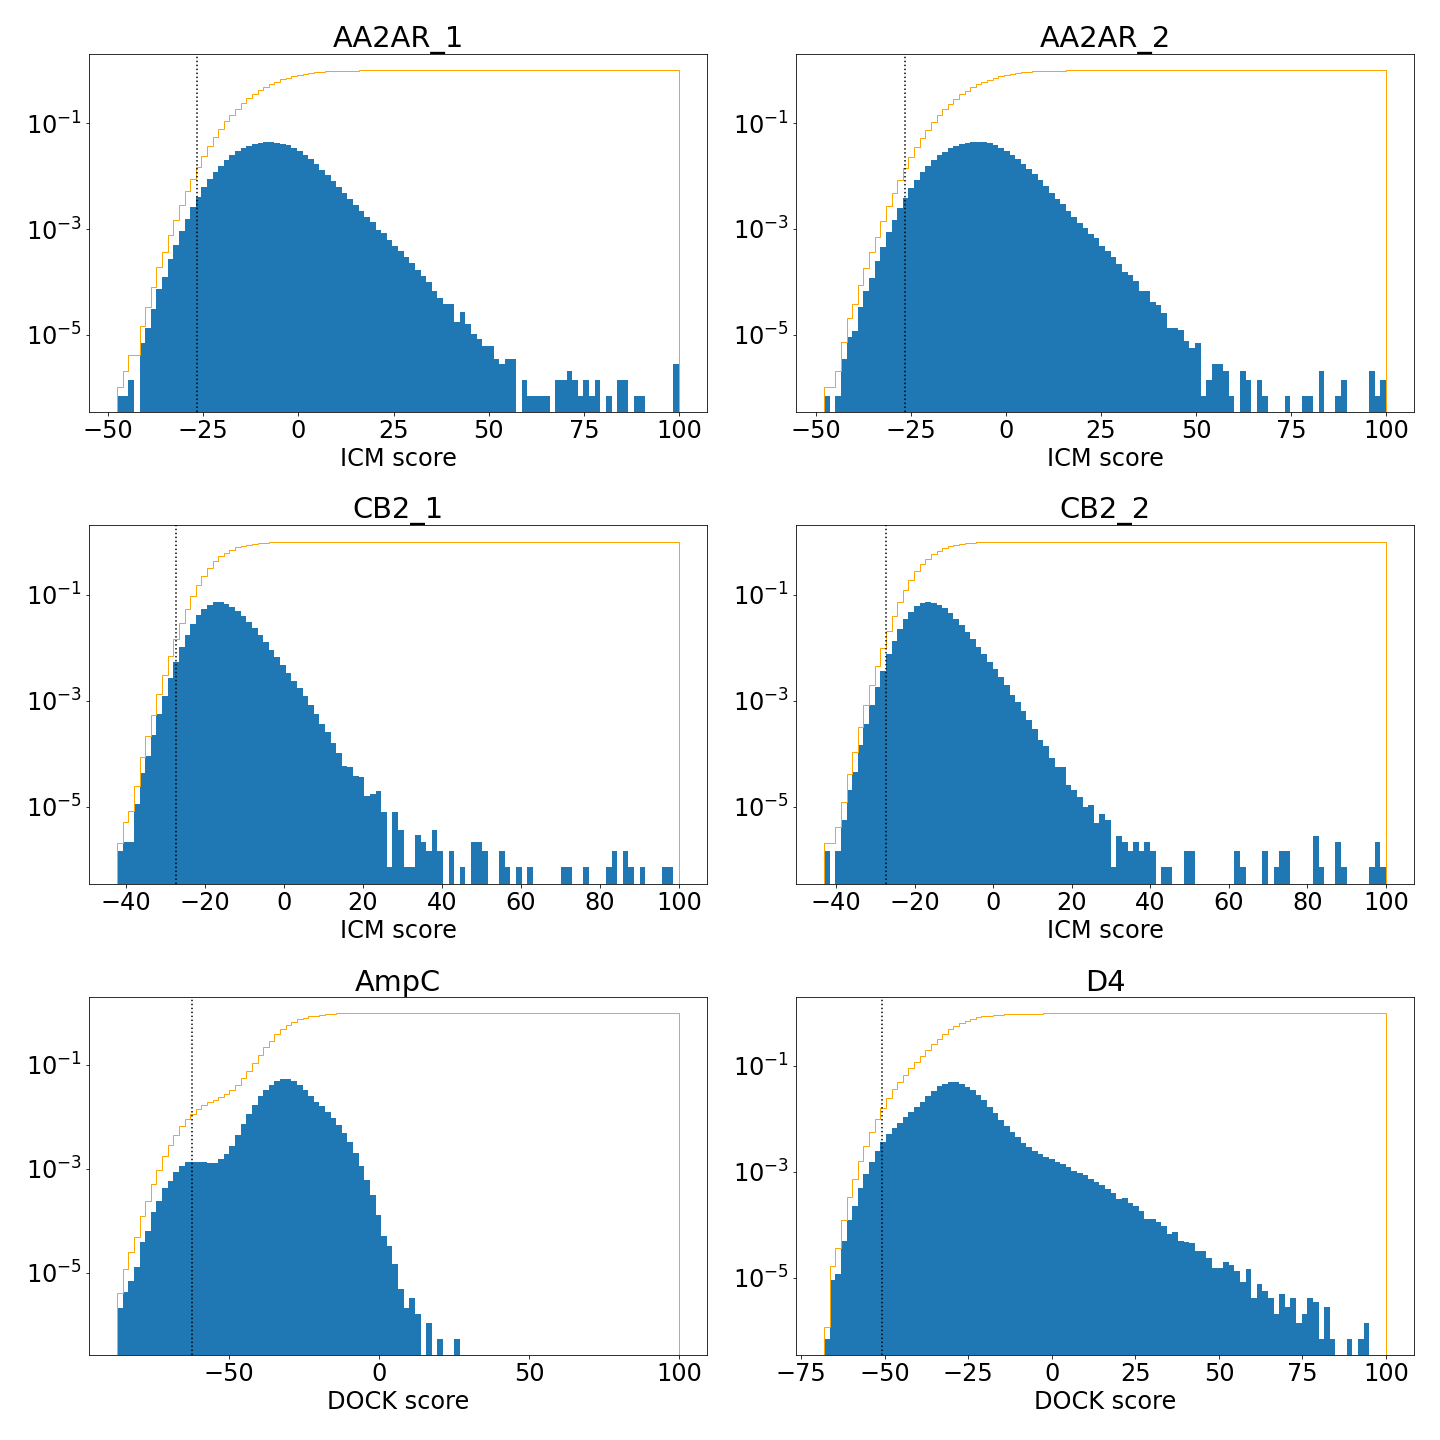
\includegraphics[width=0.8\textwidth]{figures/figure_1_scores_distribution.png}
\caption{Distributions of scores for datasets used in the study. Histogram (blue) shows log-scale score distribution, while plot (orange) shows cumulative distribution of scores. Vertical line (black) shows cutoff for top-1\% of scores.}
\label{fig:fig_1_distribution}
\end{figure}


\subsection{Single-shot prediction of virtual screening hits}
First, we tested classical ML algorithms for their ability to retrieve molecules with the best docking score without any iterations (\textit{single-shot} regime). Namely, we labeled 1\% of the top-scored ligands in datasets AmpC, D4, AA2AR\_1 and CB2\_1 as hits, and the rest as non-hits. Then we tested several ML algorithms and two baseline algorithms in their ability to recover these virtual screening hits (VSHs) from the ligand pool after training on a small subset of molecules with their scores. We choose a larger percentage, top-1\%, compared to 0.05\% in the earlier works  \cite{Graff2021AcceleratingLearning, logistic_regression, Yang2021_shoichet_active_learning} due to the small size of the library in order to decrease the subsequent deviation of the performance metric.

As for the algorithm selection, we choose both "lightweight" (linear regression and support vector machine models) and "heavyweight" (random forest, decision tree and K-neighbours models) approaches in regression mode, predicting the docking score from molecule's Morgan fingerprint directly. Namely, we tested following models (as named in scikit-learn library): LinearRegressor, Ridge/RidgeCV, LinearSVR, KNeighboursRegressor (with one and five neighbours), KNeighboursRegressor (with Jaccard metric), DecisionTreeRegressor, RandomForestRegressor, KNeighboursClassifier (with five neighbours), DecisionTreeClassifier, and SGDClassifier. All models were used with default parameters, as implemented in scikit-learn Python library \cite{scikit-learn} (ver. 0.23.2).

We used five-fold stratified cross-validation for the model performance estimation. Namely, for each train size $m$ we selected $1.2m$ ligands per each fold, labeled top-1\% as hits and used stratified five-fold split to enumerate the folds. This way, models were trained on $m$ ligands and tested on $m/5$ ligands, with $1:99$ imbalance of VSHs:non-VSHs in both train and test sets.

For performance measure, we used model recall: a number of true VSHs in top-1\% of hits, predicted by the model.

For the AA2AR and CB2 datasets we constructed lower- and upper-bound baselines to better understand the limits of our ML models. We used sampling from a Gaussian distribution, matching the overall score mean and standard deviation, as a lower-bound baseline (model "RandomGaussianRegressor"). A docking score from the second docking with the same receptor was chosen as an upper-bound baseline, assuming that no ML model can provide us with a better docking score than the docking itself (model "DockingAsPredictor"). Since the docking seed was not fixed, scores were different due to the stochastic nature of the ligand sampling \cite{abagyan_biased_1994}.

\subsection{Single-shot results extrapolation}

After obtaining the results for single-shot model performance, we explored the active learning regime. In this regime, a \textit{base model} is trained at each step, and its predictions are then docked at the next step, instead of randomly chosen ligands. 

First, we estimated the effect of batch size on the overall virtual screening performance in the active learning regime. In order to do that, we compared few scenarios: 
\begin{enumerate*}[label=(\roman*)]
    \item memory-less active learning model with LinearRegression as a base model;
    \item extrapolation of a single-shot prediction, under assumption that recall remains constant;
    \item lower-bond baseline of random docking score assignment;
    \item upper-bond baseline, picking docking score from a second docking attempt (for AA2AR and CB2 datasets).
\end{enumerate*}

In each scenario, a base learning model was initially trained on random $\texttt{batch\_size}$ ligands with their scores. This model then was used to pick the next $\texttt{batch\_size}$ ligands from the rest of the set (as top-1\% of the ligands, ranked by their predicted docking score). Then, the next base model was trained on the scores of ligands from the previous iteration, and so on.

In order to extrapolate single-shot model performance, we assumed that the model performance does not change with the deterioration of the ligand pool, and recall remains the same. Given the batch size $n$, total number of ligands $N$, recall $r$, and hits fraction $\beta=0.01$, at iteration 0 model retrieves $h_0 = n\beta$ VSHs. At iteration $j$, model retrieves fraction $r$ of the remaining VSH: $h_j = ( N\beta - \sum_{i=0}^{j-1}h_i ) \cdot r$. Subsequently, the total number of hits retrieved by step $j$ is $H_j = \sum_{i=0}^{j} h_i$.

To evaluate performance of the active learning regime, we calculated the number of retrieved VSHs. For each batch size and dataset, we performed 5 attempts, using the same fold labels among different batch sizes.

\subsection{Active learning regime parameters}

After testing the batch size effect and reliability of the constant recall extrapolation, we explored different scenarios of the active learning regime. Namely, we tried
\begin{enumerate*}[label=(\roman*)]
    \item different batch sizes ($n=8$, 40, 80, 160 and 320 thousands of ligands);
    \item exploiting models from earlier ($i < j$) iterations at iteration $j$, with different methods of ensembling of multiple models;
    \item adding previously discovered ligands to the train set at step $j$, hence making the size of the train set $X_j$ at step $j$ $|X_j| = nj$ instead of $|X_j|=n$.
\end{enumerate*}

Similarly to the previous section, we used here LinearRegression as base model, given its small training and inference time, as well as its consistently good performance on all datasets. Also, for the AA2AR and CB2 datasets, we used second docking as an upper-bond baseline. Finally, we used random score assignment as lower-bond baseline in all 4 datasets. 

Also, similarly to the previous section, we used model recall, i.e. the amount of VSHs retrieved by the active learning model, as a performance metric.

For model ensembling, we used three different regimes, summarized in figure \ref{fig:fig_2_scheme}. LastModel used no ensembling altogether, using only for the latest model predictions. MeanRank for each ligand assigned rank $p_i$ by model $i$, and used $\langle p_i \rangle$ as a ligand score. Finally, TopFromEveryModel used smaller portion of each model's top ($k$ times smaller for $k$ different models), and compiled individual tops into an ensemble prediction.


\begin{figure}[ht]
\centering
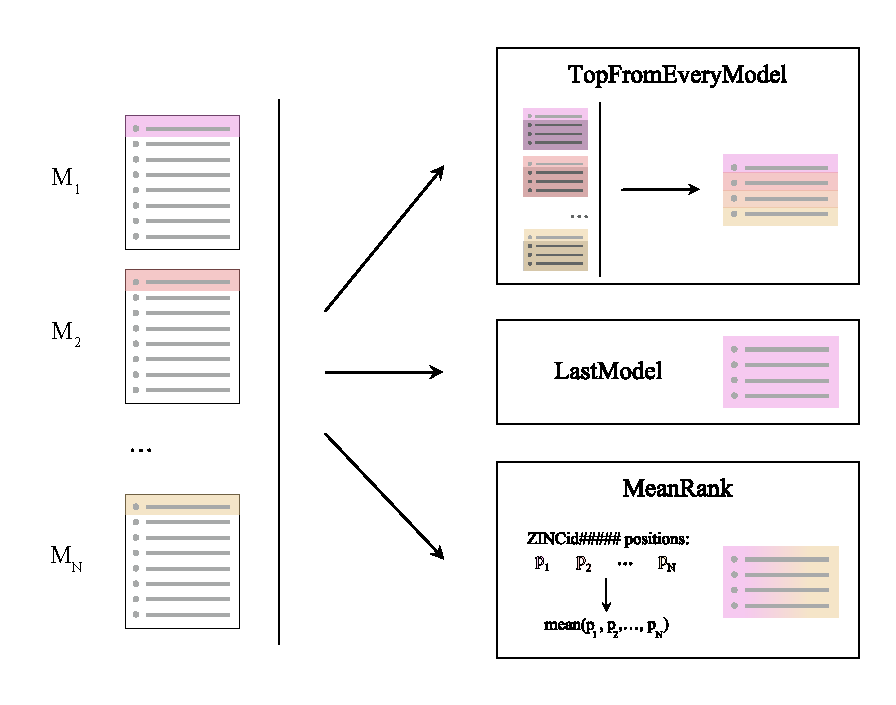
\includegraphics[width=1.0\textwidth]{figures/Figure_2_v4.pdf}
\caption{Overview of the different ensembling approaches in the active learning regime.}
\label{fig:fig_2_scheme}
\end{figure}


\subsection{Hardware}
We used a machine with 2xAMD EPYC 7502 processors @ 2.35 GHz (a total of 64 cores / 128 threads) and 256 Gb RAM for both docking and scikit-learn model training and inference.
